
%%--------------------------------------------------
%% Halliday: Fundamentals of Physics
%%--------------------------------------------------


%% Chapter 10: Rotation
%%--------------------------------------------------


%% Learning Objectives
%%--------------------------------------------------

%% 10.01: Identify that if all parts of a body rotate around a fixed axis locked together, the body is a rigid body. (This chapter is about the motion of such bodies.)
%% 10.02: Identify that the angular position of a rotating rigid body is the angle that an internal reference line makes with a fixed, external reference line.
%% 10.03: Apply the relationship between angular displacement and the initial and final angular positions.
%% 10.04: Apply the relationship between average angular velocity, angular displacement, and the time interval for that displacement.
%% 10.05: Apply the relationship between average angular acceleration, change in angular velocity, and the time interval for that change.
%% 10.06: Identify that counterclockwise motion is in the positive direction and clockwise motion is in the negative direction.
%% 10.07: Given angular position as a function of time, calculate the instantaneous angular velocity at any particular time and the average angular velocity between any two particular times.
%% 10.08: Given a graph of angular position versus time, determine the instantaneous angular velocity at a particular time and the average angular velocity between any two particular times.
%% 10.09: Identify instantaneous angular speed as the magnitude of the instantaneous angular velocity.
%% 10.10: Given angular velocity as a function of time, calculate the instantaneous angular acceleration at any particular time and the average angular acceleration between any two particular times.
%% 10.11: Given a graph of angular velocity versus time, determine the instantaneous angular acceleration at any particular time and the average angular acceleration between any two particular times.
%% 10.12: Calculate a body's change in angular velocity by integrating its angular acceleration function with respect to time.
%% 10.13: Calculate a body's change in angular position by integrating its angular velocity function with respect to time.


%% Halliday Multiple Choice Questions
%%--------------------------------------------------
\element{halliday-mc}{
\begin{question}{halliday-ch10-q01}
    A radian is about:
    \begin{multicols}{3}
    \begin{choices}
        \wrongchoice{\ang{25}}
        \wrongchoice{\ang{37}}
        \wrongchoice{\ang{45}}
      \correctchoice{\ang{57}}
        \wrongchoice{\ang{90}}
    \end{choices}
    \end{multicols}
\end{question}
}

\element{halliday-mc}{
\begin{question}{halliday-ch10-q02}
    One revolution is the same as:
    \begin{multicols}{3}
    \begin{choices}
        \wrongchoice{$1\,\si{\radian}$}
        \wrongchoice{$57\,\si{\radian}$}
        \wrongchoice{$\dfrac{\pi}{2}\,\si{\radian}$}
        \wrongchoice{$\pi\,\si{\radian}$}
      \correctchoice{$2\pi\,\si{\radian}$}
    \end{choices}
    \end{multicols}
\end{question}
}

\element{halliday-mc}{
\begin{question}{halliday-ch10-q03}
    One revolution per minute is about:
    \begin{multicols}{2}
    \begin{choices}
        \wrongchoice{\SI{0.0524}{\radian\per\second}}
      \correctchoice{\SI{0.105}{\radian\per\second}}
        \wrongchoice{\SI{0.95}{\radian\per\second}}
        \wrongchoice{\SI{1.57}{\radian\per\second}}
        \wrongchoice{\SI{6.28}{\radian\per\second}}
    \end{choices}
    \end{multicols}
\end{question}
}

\element{halliday-mc}{
\begin{question}{halliday-ch10-q04}
    If a wheel turns with constant angular speed then:
    \begin{choices}
        \wrongchoice{each point on its rim moves with constant velocity}
        \wrongchoice{each point on its rim moves with constant acceleration}
      \correctchoice{the wheel turns through equal angles in equal times}
        \wrongchoice{the angle through which the wheel turns in each second increases as time goes on}
        \wrongchoice{the angle through which the wheel turns in each second decreases as time goes on}
    \end{choices}
\end{question}
}

\element{halliday-mc}{
\begin{question}{halliday-ch10-q05}
    If a wheel is turning at \SI{3.0}{\radian\per\second},
        the time it takes to complete one revolution is about:
    \begin{multicols}{3}
    \begin{choices}
        \wrongchoice{\SI{0.33}{\second}}
        \wrongchoice{\SI{0.67}{\second}}
        \wrongchoice{\SI{1.0}{\second}}
        \wrongchoice{\SI{1.3}{\second}}
      \correctchoice{\SI{2.1}{\second}}
    \end{choices}
    \end{multicols}
\end{question}
}

\element{halliday-mc}{
\begin{question}{halliday-ch10-q06}
    If wheel turning at a constant rate completes \num{100} revolutions in \SI{10}{\second} its angular speed is:
    \begin{multicols}{3}
    \begin{choices}
        \wrongchoice{\SI{0.31}{\radian\per\second}}
        \wrongchoice{\SI{0.63}{\radian\per\second}}
        \wrongchoice{\SI{10}{\radian\per\second}}
        \wrongchoice{\SI{31}{\radian\per\second}}
      \correctchoice{\SI{63}{\radian\per\second}}
    \end{choices}
    \end{multicols}
\end{question}
}

\element{halliday-mc}{
\begin{question}{halliday-ch10-q07}
    The angular speed of the second hand of a watch is:
    \begin{multicols}{3}
    \begin{choices}
        \wrongchoice{$\dfrac{\pi}{1800}\,\si{\radian\per\second}$}
        %% changed meter to radian
        \wrongchoice{$\dfrac{\pi}{60}\,\si{\radian\per\second}$}
      \correctchoice{$\dfrac{\pi}{30}\,\si{\radian\per\second}$}
        \wrongchoice{$2\pi\,\si{\radian\per\second}$}
        \wrongchoice{$60\,\si{\radian\per\second}$}
    \end{choices}
    \end{multicols}
\end{question}
}

\element{halliday-mc}{
\begin{question}{halliday-ch10-q08}
    The angular speed of the minute hand of a watch is:
    \begin{multicols}{3}
    \begin{choices}
        %% changed meter to radian
        \wrongchoice{$\dfrac{60}{\pi}\,\si{\radian\per\second}$}
        \wrongchoice{$\dfrac{1800}{\pi}\,\si{\radian\per\second}$}
        \wrongchoice{$\pi\,\si{\radian\per\second}$}
      \correctchoice{$\dfrac{\pi}{1800}\,\si{\radian\per\second}$}
        \wrongchoice{$\dfrac{\pi}{60}\,\si{\radian\per\second}$}
    \end{choices}
    \end{multicols}
\end{question}
}

\element{halliday-mc}{
\begin{question}{halliday-ch10-q09}
    A flywheel is initially rotating at \SI{20}{\radian\per\second} and has a constant angular acceleration.
    After \SI{9.0}{\second} it has rotated through \SI{450}{\radian}.
    Its angular acceleration is:
    \begin{multicols}{2}
    \begin{choices}
        %% changed rad/s to rad/s/s
        \wrongchoice{\SI{3.3}{\radian\per\second\second}}
        \wrongchoice{\SI{4.4}{\radian\per\second\second}}
        \wrongchoice{\SI{5.6}{\radian\per\second\second}}
      \correctchoice{\SI{6.7}{\radian\per\second\second}}
        \wrongchoice{\SI{11}{\radian\per\second\second}}
    \end{choices}
    \end{multicols}
\end{question}
}

\element{halliday-mc}{
\begin{question}{halliday-ch10-q10}
    Ten seconds after an electric fan is turned on,
        the fan rotates at \SI{300}{\revolution\per\minute}.
    Its average angular acceleration is:
    \begin{multicols}{2}
    \begin{choices}
      \correctchoice{\SI{3.14}{\radian\per\second\squared}}
        \wrongchoice{\SI{30}{\radian\per\second\squared}}
        \wrongchoice{\SI{30}{\revolution\per\second\squared}}
        \wrongchoice{\SI{50}{\revolution\per\minute\squared}}
        \wrongchoice{\SI{1800}{\revolution\per\second\squared}}
    \end{choices}
    \end{multicols}
\end{question}
}

\element{halliday-mc}{
\begin{question}{halliday-ch10-q11}
    A wheel rotates with a constant angular acceleration of $\pi\,\si{\radian\per\second\squared}$.
    During a certain time interval its angular displacement is $\pi\,\si{\radian}$.
    At the end of the interval its angular velocity is $2\pi\,\si{\radian\per\second}$.
    Its angular velocity at the beginning of the interval is:
    \begin{multicols}{3}
    \begin{choices}
        \wrongchoice{zero}
        \wrongchoice{$1\,\si{\radian\per\second}$}
        \wrongchoice{$\pi\,\si{\radian\per\second}$}
      \correctchoice{$\pi\sqrt{2}\,\si{\radian\per\second}$}
        \wrongchoice{$2\pi\,\si{\radian\per\second}$}
    \end{choices}
    \end{multicols}
\end{question}
}

\element{halliday-mc}{
\begin{question}{halliday-ch10-q12}
    A flywheel rotating at \SI{12}{\revolution\per\second} is brought to rest in \SI{6}{\second}.
    The magnitude of the average angular acceleration of the wheel during this process is:
    \begin{multicols}{3}
    \begin{choices}
        \wrongchoice{$\dfrac{1}{\pi}\,\si{\radian\per\second\squared}$}
        \wrongchoice{$2\,\si{\radian\per\second\squared}$}
        \wrongchoice{$4\,\si{\radian\per\second\squared}$}
      \correctchoice{$4\pi\,\si{\radian\per\second\squared}$}
        \wrongchoice{$72\,\si{\radian\per\second\squared}$}
    \end{choices}
    \end{multicols}
\end{question}
}

\element{halliday-mc}{
\begin{question}{halliday-ch10-q13}
    A phonograph turntable, initially rotating at \SI{0.75}{\revolution\per\second},
        slows down and stops in \SI{30}{\second}.
    The magnitude of its average angular acceleration for this process is:
    \begin{multicols}{3}
    \begin{choices}
        \wrongchoice{$\dfrac{3}{2}\,\si{\radian\per\second\squared}$}
        \wrongchoice{$\dfrac{3\pi}{2}\,\si{\radian\per\second\squared}$}
        \wrongchoice{$\dfrac{\pi}{40}\,\si{\radian\per\second\squared}$}
      \correctchoice{$\dfrac{\pi}{20}\,\si{\radian\per\second\squared}$}
        \wrongchoice{$\dfrac{3}{4}\,\si{\radian\per\second\squared}$}
    \end{choices}
    \end{multicols}
\end{question}
}

\element{halliday-mc}{
\begin{question}{halliday-ch10-q14}
    The angular velocity of a rotating wheel increases by \SI{2}{\revolution\second} every minute.
    The angular acceleration of this wheel is:
    \begin{multicols}{3}
    \begin{choices}
        \wrongchoice{$4\pi^2\,\si{\radian\per\second\squared}$}
        \wrongchoice{$2\pi\,\si{\radian\per\second\squared}$}
        \wrongchoice{$\dfrac{1}{30}\,\si{\radian\per\second\squared}$}
      \correctchoice{$\dfrac{\pi}{15}\,\si{\radian\per\second\squared}$}
        \wrongchoice{$4\pi\,\si{\radian\per\second\squared}$}
    \end{choices}
    \end{multicols}
\end{question}
}

\element{halliday-mc}{
\begin{question}{halliday-ch10-q15}
    A wheel initially has an angular velocity of \SI{18}{\radian\per\second}.
    It has a constant angular acceleration of \SI{2.0}{\radian\per\second} and is slowing at first.
    What time elapses before its angular velocity is \SI{18}{\radian\per\second} in the direction opposite to its initial angular velocity?
    \begin{multicols}{3}
    \begin{choices}
        \wrongchoice{\SI{3.0}{\second}}
        \wrongchoice{\SI{6.0}{\second}}
        \wrongchoice{\SI{9.0}{\second}}
      \correctchoice{\SI{18}{\second}}
        \wrongchoice{\SI{36}{\second}}
    \end{choices}
    \end{multicols}
\end{question}
}

\element{halliday-mc}{
\begin{question}{halliday-ch10-q16}
    A wheel initially has an angular velocity of \SI{36}{\radian\per\second} but after \SI{6.0}{\second} its angular velocity is \SI{24}{\radian\per\second}.
    If its angular acceleration is constant its value is:
    \begin{multicols}{2}
    \begin{choices}
        \wrongchoice{\SI{2.0}{\radian\per\second\squared}}
      \correctchoice{\SI{-2.0}{\radian\per\second\squared}}
        \wrongchoice{\SI{3.0}{\radian\per\second\squared}}
        \wrongchoice{\SI{-3.0}{\radian\per\second\squared}}
        \wrongchoice{\SI{6.0}{\radian\per\second\squared}}
    \end{choices}
    \end{multicols}
\end{question}
}

\element{halliday-mc}{
\begin{question}{halliday-ch10-q17}
    A wheel initially has an angular velocity of \SI{-36}{\radian\per\second} but after \SI{6.0}{\second} its angular velocity is \SI{-24}{\radian\per\second}.
    If its angular acceleration is constant the value is:
    \begin{multicols}{2}
    \begin{choices}
      \correctchoice{\SI{2.0}{\radian\per\second\squared}}
        \wrongchoice{\SI{-2.0}{\radian\per\second\squared}}
        \wrongchoice{\SI{3.0}{\radian\per\second\squared}}
        \wrongchoice{\SI{-3.0}{\radian\per\second\squared}}
        \wrongchoice{\SI{-6.0}{\radian\per\second\squared}}
    \end{choices}
    \end{multicols}
\end{question}
}

\element{halliday-mc}{
\begin{question}{halliday-ch10-q18}
    A wheel initially has an angular velocity of \SI{18}{\radian\per\second} but it is slowing at a rate of \SI{2.0}{\radian\per\second\squared}.
    By the time it stops it will have turned through:
    \begin{multicols}{3}
    \begin{choices}
      \correctchoice{\SI{81}{\radian}}
        \wrongchoice{\SI{160}{\radian}}
        \wrongchoice{\SI{245}{\radian}}
        \wrongchoice{\SI{330}{\radian}}
        \wrongchoice{\SI{410}{\radian}}
    \end{choices}
    \end{multicols}
\end{question}
}

\element{halliday-mc}{
\begin{question}{halliday-ch10-q19}
    A wheel starts from rest and has an angular acceleration of \SI{4.0}{\radian\per\second\squared}.
    When it has made \SI{10}{\revolution} its angular velocity is:
    \begin{multicols}{3}
    \begin{choices}
        \wrongchoice{\SI{16}{\radian\per\second}}
        \wrongchoice{\SI{22}{\radian\per\second}}
        \wrongchoice{\SI{32}{\radian\per\second}}
        \wrongchoice{\SI{250}{\radian\per\second}}
        \wrongchoice{\SI{500}{\radian\per\second}}
    \end{choices}
    \end{multicols}
\end{question}
}

\element{halliday-mc}{
\begin{question}{halliday-ch10-q20}
    A wheel starts from rest and has an angular acceleration of \SI{4.0}{\radian\per\second\squared}.
    The time it takes to make \SI{10}{\revolution} is:
    \begin{multicols}{3}
    \begin{choices}
        \wrongchoice{\SI{0.50}{\second}}
        \wrongchoice{\SI{0.71}{\second}}
        \wrongchoice{\SI{2.2}{\second}}
        \wrongchoice{\SI{2.8}{\second}}
      \correctchoice{\SI{5.6}{\second}}
    \end{choices}
    \end{multicols}
\end{question}
}

\element{halliday-mc}{
\begin{question}{halliday-ch10-q21}
    A wheel starts from rest and has an angular acceleration that is given by $\alpha\left(t\right) = \left(\SI{6}{\radian\per\second\tothefourth}\right) t^2$.
    The angle through which it turns in time $t$ is given by:
    \begin{multicols}{2}
    \begin{choices}
        \wrongchoice{$\left(\dfrac{1}{8}t^4\right)\,\si{\radian}$}
        \wrongchoice{$\left(\dfrac{1}{4}t^4\right)\,\si{\radian}$}
      \correctchoice{$\left(\dfrac{1}{2}t^4\right)\,\si{\radian}$}
        \wrongchoice{$\left(t^4\right)\,\si{\radian}$}
        \wrongchoice{\SI{12}{\radian}}
    \end{choices}
    \end{multicols}
\end{question}
}

\element{halliday-mc}{
\begin{question}{halliday-ch10-q22}
    A wheel starts from rest and has an angular acceleration that is given by $\alpha\left(t\right) = \left(\SI{6.0}{\radian\per\second\tothefourth}\right) t^2$.
    The time it takes to make \SI{10}{\revolution} is:
    \begin{multicols}{3}
    \begin{choices}
        \wrongchoice{\SI{2.8}{\second}}
      \correctchoice{\SI{3.3}{\second}}
        \wrongchoice{\SI{4.0}{\second}}
        \wrongchoice{\SI{4.7}{\second}}
        \wrongchoice{\SI{5.3}{\second}}
    \end{choices}
    \end{multicols}
\end{question}
}

\element{halliday-mc}{
\begin{question}{halliday-ch10-q23}
    A wheel starts from rest and has an angular acceleration that is given by $\alpha\left(t\right) = \left(\SI{6.0}{\radian\per\second\tothefourth}\right) t^2$.
    After it has turned through \SI{10}{\revolution} its angular velocity is:
    \begin{multicols}{3}
    \begin{choices}
        \wrongchoice{\SI{63}{\radian\per\second}}
      \correctchoice{\SI{75}{\radian\per\second}}
        \wrongchoice{\SI{89}{\radian\per\second}}
        \wrongchoice{\SI{130}{\radian\per\second}}
        \wrongchoice{\SI{210}{\radian\per\second}}
    \end{choices}
    \end{multicols}
\end{question}
}

\element{halliday-mc}{
\begin{question}{halliday-ch10-q24}
    A wheel is spinning at \SI{27}{\radian\per\second} but is slowing with an angular acceleration that has a magnitude given by $\left(\SI{3.0}{\radian\per\second\tothefourth}\right) t^2$.
    It stops in a time of:
    \begin{multicols}{3}
    \begin{choices}
        \wrongchoice{\SI{1.7}{\second}}
        \wrongchoice{\SI{2.6}{\second}}
      \correctchoice{\SI{3.0}{\second}}
        \wrongchoice{\SI{4.4}{\second}}
        \wrongchoice{\SI{7.3}{\second}}
    \end{choices}
    \end{multicols}
\end{question}
}

\element{halliday-mc}{
\begin{question}{halliday-ch10-q25}
    If the angular velocity vector of a spinning body points out of the page then,
        when viewed from above the page, the body is spinning:
    \begin{choices}
        \wrongchoice{clockwise about an axis that is perpendicular to the page}
      \correctchoice{counterclockwise about an axis that is perpendicular to the page}
        \wrongchoice{about an axis that is parallel to the page}
        \wrongchoice{about an axis that is changing orientation}
        \wrongchoice{about an axis that is getting longer}
    \end{choices}
\end{question}
}

\element{halliday-mc}{
\begin{question}{halliday-ch10-q26}
    The angular velocity vector of a spinning body points out of the page.
    If the angular acceleration vector points into the page then:
    \begin{choices}
      \correctchoice{the body is slowing down}
        \wrongchoice{the body is speeding up}
        \wrongchoice{the body is starting to turn in the opposite direction}
        \wrongchoice{the axis of rotation is changing orientation}
        \wrongchoice{none of the provided}
    \end{choices}
\end{question}
}

\element{halliday-mc}{
\begin{question}{halliday-ch10-q27}
    A child, riding on a large merry-go-round,
        travels a distance of \SI{3000}{\meter} in a circle of diameter \SI{40}{\meter}.
    The total angle through which she revolves is:
    \begin{multicols}{2}
    \begin{choices}
        \wrongchoice{\SI{50}{\radian}}
        \wrongchoice{\SI{75}{\radian}}
      \correctchoice{\SI{150}{\radian}}
        \wrongchoice{\SI{314}{\radian}}
        \wrongchoice{none of the provided}
    \end{choices}
    \end{multicols}
\end{question}
}

\element{halliday-mc}{
\begin{question}{halliday-ch10-q28}
    The figure shows a cylinder of radius \SI{0.7}{\meter} rotating about its axis at \SI{10}{\radian\per\second}.
    \begin{center}
    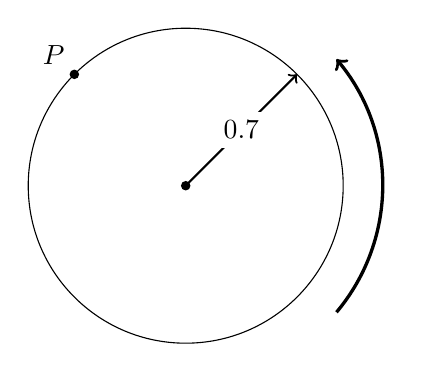
\begin{tikzpicture}
        \draw[fill] (0,0) circle (1.5pt);
        \draw (0,0) circle (2cm);
        \draw[thick,->] (0,0) -- (45:2cm) node[pos=0.5,anchor=center,fill=white] {\SI{0.7}{\meter}};
        \draw[very thick,->] (-40:2.5) arc(-40:40:2.5);
        \draw[fill] (135:2) circle (1.5pt) node[anchor=south east] {$P$};
    \end{tikzpicture}
    \end{center}
    The speed of the point $P$ is:
    \begin{multicols}{2}
    \begin{choices}
      \correctchoice{\SI{7.0}{\meter\per\second}}
        \wrongchoice{\SI[parse-numbers=false]{14\pi}{\radian\per\second}}
        \wrongchoice{\SI[parse-numbers=false]{7.0\pi}{\radian\per\second}}
        \wrongchoice{\SI{0.70}{\meter\per\second}}
        \wrongchoice{none of the provided}
    \end{choices}
    \end{multicols}
\end{question}
}

\element{halliday-mc}{
\begin{question}{halliday-ch10-q29}
    The fan shown has been turned on and is now slowing as it rotates clockwise.
    \begin{center}
    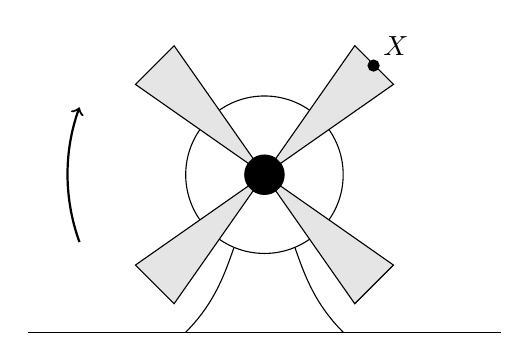
\begin{tikzpicture}
        %% Floor and Base
        \draw (-3,-2) -- (+3,-2);
        \draw (-1,-2) to[out=45,in=240] (0,0);
        \draw (+1,-2) to[out=135,in=300] (0,0);
        %% Casing
        \draw[fill=white] (0,0) circle (1cm);
        \draw[fill] (0,0) circle (0.25cm);
        %% Blades
        \draw[fill=white!90!black] (35:0.25) -- (35:2) -- (55:2) -- (55:0.25) --cycle;
        \draw[fill=white!90!black] (125:0.25) -- (125:2) -- (145:2) -- (145:0.25) --cycle;
        \draw[fill=white!90!black] (215:0.25) -- (215:2) -- (235:2) -- (235:0.25) --cycle;
        \draw[fill=white!90!black] (325:0.25) -- (325:2) -- (305:2) -- (305:0.25) --cycle;
        %% Labels
        \draw[fill] (45:1.96) circle (2pt) node[anchor=south west] {$X$};
        \draw[thick,->] (200:2.5) arc(200:160:2.5);
    \end{tikzpicture}
    \end{center}
    The direction of the acceleration of the point $X$ on the fan tip could be:
    \begin{multicols}{3}
    \begin{choices}
        \AMCboxDimensions{down=-0.4cm}
        \wrongchoice{
            \begin{tikzpicture}
                \draw[white] (0,0) rectangle (1,1);
                \draw[thick,->] (0.85,0.85) -- ++(225:1);
            \end{tikzpicture}
        }
        \wrongchoice{
            \begin{tikzpicture}
                \draw[white] (0,0) rectangle (1,1);
                \draw[thick,->] (0.15,0.85) -- ++(-45:1);
            \end{tikzpicture}
        }
        \wrongchoice{
            \begin{tikzpicture}
                \draw[white] (0,0) rectangle (1,1);
                \draw[thick,->] (0.5,1) -- ++(270:1);
            \end{tikzpicture}
        }
        %% ANS is D
        \correctchoice{
            \begin{tikzpicture}
                \draw[white] (0,0) rectangle (1,1);
                \draw[thick,->] (1,0.5) -- ++(180:1);
            \end{tikzpicture}
        }
        \wrongchoice{
            \begin{tikzpicture}
                \draw[white] (0,0) rectangle (1,1);
                \draw[thick,->] (0.5,0) -- ++(90:1);
            \end{tikzpicture}
        }
    \end{choices}
    \end{multicols}
\end{question}
}

\element{halliday-mc}{
\begin{question}{halliday-ch10-q30}
    A wheel of diameter \SI{3.0}{\centi\meter} has a \SI{4.0}{\meter} cord wrapped around its periphery.
    Starting from rest, the wheel is given a constant angular acceleration of \SI{2.0}{\radian\per\second}.
    The cord will unwind in:
    \begin{multicols}{3}
    \begin{choices}
        \wrongchoice{\SI{0.82}{\second}}
        \wrongchoice{\SI{2.0}{\second}}
        \wrongchoice{\SI{8.0}{\second}}
      \correctchoice{\SI{16}{\second}}
        \wrongchoice{\SI{130}{\second}}
    \end{choices}
    \end{multicols}
\end{question}
}

\element{halliday-mc}{
\begin{question}{halliday-ch10-q31}
    A particle moves in a circular path of radius \SI{0.10}{\meter} with a constant angular speed of \SI{5}{\revolution\per\second}.
    The acceleration of the particle is:
    \begin{multicols}{2}
    \begin{choices}
        \wrongchoice{\SI[parse-numbers=false]{0.10\pi}{\meter\per\second\squared}}
        \wrongchoice{\SI[parse-numbers=false]{0.50}{\meter\per\second\squared}}
        \wrongchoice{\SI[parse-numbers=false]{500\pi}{\meter\per\second\squared}}
        \wrongchoice{\SI[parse-numbers=false]{1000\pi^2}{\meter\per\second\squared}}
      \correctchoice{\SI[parse-numbers=false]{10\pi^2}{\meter\per\second\squared}}
    \end{choices}
    \end{multicols}
\end{question}
}

\element{halliday-mc}{
\begin{question}{halliday-ch10-q32}
    A car travels north at constant velocity.
    It goes over a piece of mud,
        which sticks to the tire.
    The initial acceleration of the mud,
        as it leaves the ground, is:
    \begin{choices}
      \correctchoice{vertically upward}
        \wrongchoice{horizontally to the north}
        \wrongchoice{horizontally to the south}
        \wrongchoice{zero}
        \wrongchoice{upward and forward at \ang{45} to the horizontal}
    \end{choices}
\end{question}
}

\element{halliday-mc}{
\begin{question}{halliday-ch10-q33}
    Wrapping paper is being from a \SI{5.0}{\centi\meter} radius tube,
        free to rotate on its axis.
    If it is pulled at the constant rate of \SI{10}{\centi\meter\per\second} and does not slip on the tube,
        the angular velocity of the tube is:
    \begin{multicols}{2}
    \begin{choices}
      \correctchoice{\SI{2.0}{\radian\per\second}}
        \wrongchoice{\SI{5.0}{\radian\per\second}}
        \wrongchoice{\SI{10}{\radian\per\second}}
        \wrongchoice{\SI{25}{\radian\per\second}}
        \wrongchoice{\SI{50}{\radian\per\second}}
    \end{choices}
    \end{multicols}
\end{question}
}

\element{halliday-mc}{
\begin{question}{halliday-ch10-q34}
    String is wrapped around the periphery of a \SI{5.0}{\centi\meter} radius cylinder,
        free to rotate on its axis.
    The string is pulled straight out at a constant rate of \SI{10}{\centi\meter\per\second}
        and does not slip on the cylinder.
    As each small segment of string leaves the cylinder,
        its acceleration changes by:
    \begin{multicols}{2}
    \begin{choices}
        \wrongchoice{zero}
        \wrongchoice{\SI{0.010}{\meter\per\second\squared}}
        \wrongchoice{\SI{0.020}{\meter\per\second\squared}}
        \wrongchoice{\SI{0.10}{\meter\per\second\squared}}
      \correctchoice{\SI{0.20}{\meter\per\second\squared}}
    \end{choices}
    \end{multicols}
\end{question}
}

\element{halliday-mc}{
\begin{question}{halliday-ch10-q35}
    A flywheel of diameter \SI{1.2}{\meter} has a constant angular acceleration of \SI{5.0}{\radian\per\second\squared}.
    The tangential acceleration of a point on its rim is:
    \begin{multicols}{2}
    \begin{choices}
        \wrongchoice{\SI{5.0}{\radian\per\second\squared}}
      \correctchoice{\SI{3.0}{\meter\per\second\squared}}
        \wrongchoice{\SI{5.0}{\meter\per\second\squared}}
        \wrongchoice{\SI{6.0}{\meter\per\second\squared}}
        \wrongchoice{\SI{12}{\meter\per\second\squared}}
    \end{choices}
    \end{multicols}
\end{question}
}

\element{halliday-mc}{
\begin{question}{halliday-ch10-q36}
    For a wheel spinning with constant angular acceleration on an axis through its center,
        the ratio of the speed of a point on the rim to the speed of a point halfway between the center and the rim is:
    \begin{multicols}{3}
    \begin{choices}
        \wrongchoice{\num{1}}
      \correctchoice{\num{2}}
        \wrongchoice{\num{1/2}}
        \wrongchoice{\num{4}}
        \wrongchoice{\num{1/4}}
    \end{choices}
    \end{multicols}
\end{question}
}

\element{halliday-mc}{
\begin{question}{halliday-ch10-q37}
    For a wheel spinning on an axis through its center,
        the ratio of the tangential acceleration of a point on the rim to the tangential acceleration of a point halfway between the center and the rim is:
    \begin{multicols}{3}
    \begin{choices}
        \wrongchoice{\num{1}}
      \correctchoice{\num{2}}
        \wrongchoice{\num{1/2}}
        \wrongchoice{\num{4}}
        \wrongchoice{\num{1/4}}
    \end{choices}
    \end{multicols}
\end{question}
}

\element{halliday-mc}{
\begin{question}{halliday-ch10-q38}
    For a wheel spinning on an axis through its center,
        the ratio of the radial acceleration of a point on the rim to the radial acceleration of a point halfway between the center and the rim is:
    \begin{multicols}{3}
    \begin{choices}
        \wrongchoice{\num{1}}
      \correctchoice{\num{2}}
        \wrongchoice{\num{1/2}}
        \wrongchoice{\num{4}}
        \wrongchoice{\num{1/4}}
    \end{choices}
    \end{multicols}
\end{question}
}

\element{halliday-mc}{
\begin{question}{halliday-ch10-q39}
    Two wheels are identical but wheel $B$ is spinning with twice the angular speed of wheel $A$.
    The ratio of the magnitude of the radial acceleration of a point on the rim of $B$ to the magnitude of the radial acceleration of a point on the rim of $A$ is:
    \begin{multicols}{3}
    \begin{choices}
        \wrongchoice{\num{1}}
        \wrongchoice{\num{2}}
        \wrongchoice{\num{1/2}}
      \correctchoice{\num{4}}
        \wrongchoice{\num{1/4}}
    \end{choices}
    \end{multicols}
\end{question}
}

\element{halliday-mc}{
\begin{question}{halliday-ch10-q40}
    A wheel starts from rest and spins with a constant angular acceleration.
    As time goes on the acceleration vector for a point on the rim:
    \begin{choices}
        \wrongchoice{decreases in magnitude and becomes more nearly tangent to the rim}
        \wrongchoice{decreases in magnitude and becomes more early radial}
        \wrongchoice{increases in magnitude and becomes more nearly tangent to the rim}
      \correctchoice{increases in magnitude and becomes more nearly radial}
        \wrongchoice{increases in magnitude but retains the same angle with the tangent to the rim}
    \end{choices}
\end{question}
}

\element{halliday-mc}{
\begin{question}{halliday-ch10-q41}
    The magnitude of the acceleration of a point on a spinning wheel is increased by a factor of 4 if:
    \begin{choices}
        \wrongchoice{the magnitudes of the angular velocity and the angular acceleration are each multiplied by a factor of 4}
        \wrongchoice{the magnitude of the angular velocity is multiplied by a factor of 4 and the angular accel- eration is not changed}
        \wrongchoice{the magnitudes of the angular velocity and the angular acceleration are each multiplied by a factor of 2}
        \wrongchoice{the magnitude of the angular velocity is multiplied by a factor of 2 and the angular accel- eration is not changed}
      \correctchoice{the magnitude of the angular velocity is multiplied by a factor of 2 and the magnitude of the angular acceleration is multiplied by a factor of 4}
    \end{choices}
\end{question}
}

\element{halliday-mc}{
\begin{question}{halliday-ch10-q42}
    Three identical balls are tied by light strings to the same rod and rotate around it,
        as shown below.
    \begin{center}
    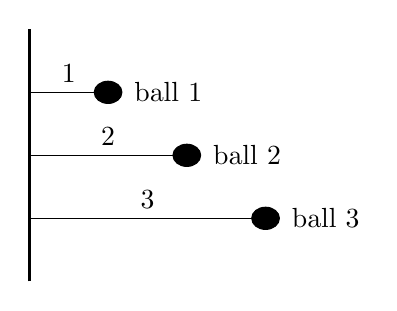
\begin{tikzpicture}[yscale=0.8]
        \draw[very thick] (0,-1) -- (0,3);
        %% Ball 3
        \draw (0,0) -- (3,0) node[pos=0.5,anchor=south] {\SI{3}{\meter}};
        \draw[fill] (3,0) circle (5pt) node[anchor=west,xshift=6pt] {ball 3};
        %% Ball 2
        \draw (0,1) -- (2,1) node[pos=0.5,anchor=south] {\SI{2}{\meter}};
        \draw[fill] (2,1) circle (5pt) node[anchor=west,xshift=6pt] {ball 2};
        %% Ball 1
        \draw (0,2) -- (1,2) node[pos=0.5,anchor=south] {\SI{1}{\meter}};
        \draw[fill] (1,2) circle (5pt) node[anchor=west,xshift=6pt] {ball 1};
    \end{tikzpicture}
    \end{center}
    Rank the balls according to their rotational inertia,
        least to greatest.
    \begin{multicols}{2}
    \begin{choices}
      \correctchoice{1, 2, 3}
        \wrongchoice{3, 2, 1}
        \wrongchoice{3, then 1 and 2 tie}
        \wrongchoice{1, 3, 2}
        \wrongchoice{All are the same}
    \end{choices}
    \end{multicols}
\end{question}
}

\element{halliday-mc}{
\begin{question}{halliday-ch10-q43}
    Four identical particles, each with mass $m$,
        are arranged in the $x$, $y$ plane as shown.
    They are connected by light sticks to form a rigid body.
    \begin{center}
    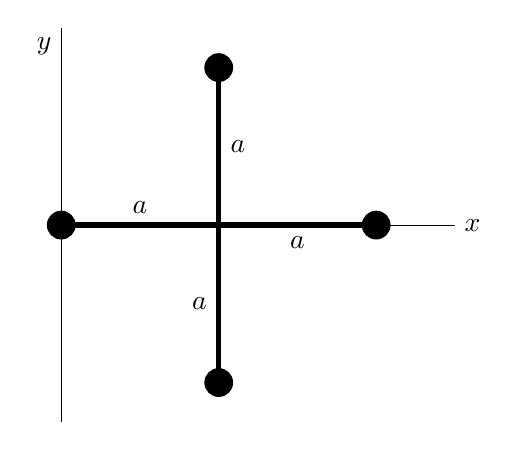
\begin{tikzpicture}
        %% X and Y axis
        \draw (0,-2.5) -- (0,2.5) node[anchor=north east] {$y$};
        \draw (0,0) -- (5,0) node[anchor=west] {$x$};
        %% horizontal balls
        \draw[fill] (0,0) circle (5pt);
        \draw[fill] (4,0) circle (5pt);
        %% vertical balls
        \draw[fill] (2,+2) circle (5pt);
        \draw[fill] (2,-2) circle (5pt);
        %% connecting rods
        \draw[line width=2pt] (0,0) -- (4,0)
            node[pos=0.25,anchor=south] {$a$}
            node[pos=0.75,anchor=north] {$a$};
        \draw[line width=2pt] (2,-2) -- (2,+2)
            node[pos=0.25,anchor=east] {$a$}
            node[pos=0.75,anchor=west] {$a$};
        %% NOTE: indication of rotation direction?
    \end{tikzpicture}
    \end{center}
    If $m=\SI{2.0}{\kilo\gram}$ and $a=\SI{1.0}{\meter}$,
        the rotational inertia of this array about the $y$ axis is:
    \begin{multicols}{2}
    \begin{choices}
        \wrongchoice{\SI{4.0}{\kilo\gram\meter\squared}}
      \correctchoice{\SI{12}{\kilo\gram\meter\squared}}
        \wrongchoice{\SI{9.6}{\kilo\gram\meter\squared}}
        \wrongchoice{\SI{4.8}{\kilo\gram\meter\squared}}
        \wrongchoice{none of the provided}
    \end{choices}
    \end{multicols}
\end{question}
}

\element{halliday-mc}{
\begin{question}{halliday-ch10-q44}
    Three identical balls, with masses of $M$, $2M$, and $3M$,
        are fastened to a massless rod of length $L$ as shown.
    \begin{center}
    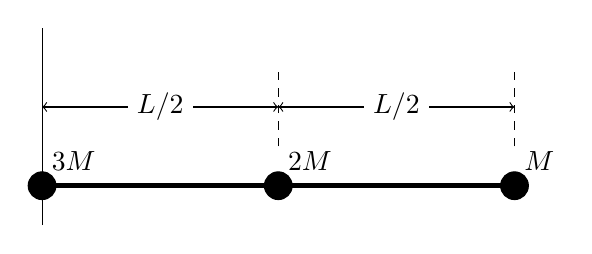
\begin{tikzpicture}
        %% Labels
        \draw (0,-0.5) -- (0,+2);
        \draw[dashed] (3,0.5) -- (3,1.5);
        \draw[dashed] (6,0.5) -- (6,1.5);
        \draw[<->] (0,1) -- (3,1) node[pos=0.5,anchor=center,fill=white] {$L/2$};
        \draw[<->] (3,1) -- (6,1) node[pos=0.5,anchor=center,fill=white] {$L/2$};
        %% Balls
        \draw[fill] (0,0) circle (5pt) node[anchor=south west,yshift=2pt] {$3M$};
        \draw[fill] (3,0) circle (5pt) node[anchor=south west,yshift=2pt] {$2M$};
        \draw[fill] (6,0) circle (5pt) node[anchor=south west,yshift=2pt] {$M$};
        \draw[line width=2pt] (0,0) -- (6,0);
    \end{tikzpicture}
    \end{center}
    The rotational inertia about the left end of the rod is:
    \begin{multicols}{3}
    \begin{choices}
        \wrongchoice{$\dfrac{M L^2}{2}$}
        \wrongchoice{$M L^2$}
        \wrongchoice{$\dfrac{3M L^2}{2}$}
        \wrongchoice{$6M L^2$}
      \correctchoice{$\dfrac{3M L^2}{4}$}
    \end{choices}
    \end{multicols}
\end{question}
}

\element{halliday-mc}{
\begin{question}{halliday-ch10-q45}
    The rotational inertia of a thin cylindrical shell of mass $M$,
        radius $R$, and length $L$ about its central axis $\left(X-X^{\prime}\right)$ is:
    \begin{center}
    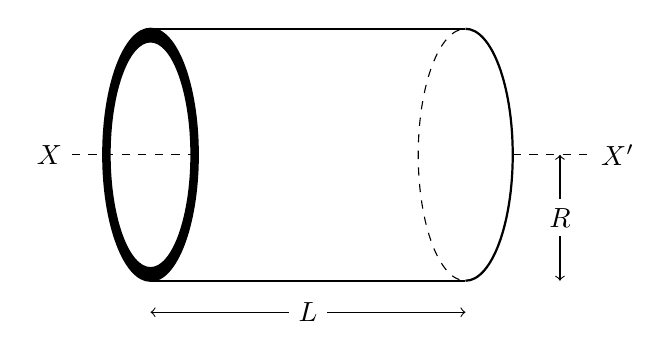
\begin{tikzpicture}[scale=0.8]
        %% Barrel
        \draw[thick,fill] (0,0) circle (0.75cm and 2cm);
        \draw[thick,fill=white] (0,0) circle (0.65cm and 1.8cm);
        \draw[dashed] (5,0) circle (0.75cm and 2cm);
        \draw[thick] (5,-2) arc (-90:90:0.75cm and 2cm);
        \draw[thick] (0,2) -- (5,2);
        \draw[thick] (0,-2) -- (5,-2);
        %% Labels
        \draw[dashed] (-1.25,0) -- (0.75,0) node[pos=0.0,anchor=east] {$X$};
        \draw[dashed] (5.75,0) -- (7.0,0) node[pos=1.0,anchor=west] {$X^{\prime}$};
        \draw[<->] (6.5,0) -- (6.5,-2) node[pos=0.5,anchor=center,fill=white] {$R$};
        \draw[<->] (0,-2.5) -- (5,-2.5) node[pos=0.5,anchor=center,fill=white] {$L$};
    \end{tikzpicture}
    \end{center}
    \begin{multicols}{2}
    \begin{choices}
        \wrongchoice{$\dfrac{M R^2}{2}$}
        \wrongchoice{$\dfrac{M L^2}{2}$}
        \wrongchoice{$M L^2$}
      \correctchoice{$M R^2$}
        \wrongchoice{none of the provided}
    \end{choices}
    \end{multicols}
\end{question}
}

\element{halliday-mc}{
\begin{question}{halliday-ch10-q46}
    The rotational inertia of a wheel about its axle does not depend upon its:
    \begin{choices}
        \wrongchoice{diameter}
        \wrongchoice{mass}
        \wrongchoice{distribution of mass}
      \correctchoice{speed of rotation}
        \wrongchoice{material composition}
    \end{choices}
\end{question}
}

\element{halliday-mc}{
\begin{question}{halliday-ch10-q47}
    Consider four objects, each having the same mass and the same radius:
    \begin{enumerate}
        \item a solid sphere
        \item a hollow sphere
        \item a flat disk in the $x$, $y$ plane
        \item a hoop in the $x$, $y$ plane
    \end{enumerate}
    The order of increasing rotational inertia about an axis through
        the center of mass and parallel to the $z$ axis is:
    \begin{multicols}{2}
    \begin{choices}
        \wrongchoice{1, 2, 3, 4}
        \wrongchoice{4, 3, 2, 1}
      \correctchoice{1, 3, 2, 4}
        \wrongchoice{4, 2, 3, 1}
        \wrongchoice{3, 1, 2, 4}
    \end{choices}
    \end{multicols}
\end{question}
}

\element{halliday-mc}{
\begin{question}{halliday-ch10-q48}
    $A$ and $B$ are two solid cylinders made of aluminum.
    Their dimensions are shown.
    \begin{center}
    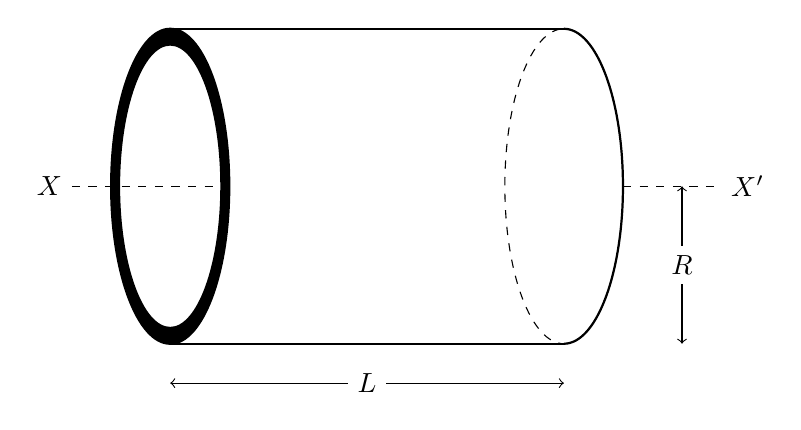
\begin{tikzpicture}
        %% NOTE: TODO: finish this
        %% NOTE: Two scopes and shift each??
        %% Barrel
        \draw[thick,fill] (0,0) circle (0.75cm and 2cm);
        \draw[thick,fill=white] (0,0) circle (0.65cm and 1.8cm);
        \draw[dashed] (5,0) circle (0.75cm and 2cm);
        \draw[thick] (5,-2) arc (-90:90:0.75cm and 2cm);
        \draw[thick] (0,2) -- (5,2);
        \draw[thick] (0,-2) -- (5,-2);
        %% Labels
        \draw[dashed] (-1.25,0) -- (0.75,0) node[pos=0.0,anchor=east] {$X$};
        \draw[dashed] (5.75,0) -- (7.0,0) node[pos=1.0,anchor=west] {$X^{\prime}$};
        \draw[<->] (6.5,0) -- (6.5,-2) node[pos=0.5,anchor=center,fill=white] {$R$};
        \draw[<->] (0,-2.5) -- (5,-2.5) node[pos=0.5,anchor=center,fill=white] {$L$};
    \end{tikzpicture}
    \end{center}
    The ratio of the rotational inertia of $B$ to that of $A$ about the common axis $X-X^{\prime}$ is:
    \begin{multicols}{3}
    \begin{choices}
        \wrongchoice{\num{2}}
        \wrongchoice{\num{4}}
        \wrongchoice{\num{8}}
        \wrongchoice{\num{16}}
        \wrongchoice{\num{32}}
    \end{choices}
    \end{multicols}
\end{question}
}

\element{halliday-mc}{
\begin{question}{halliday-ch10-q49}
    Two uniform circular disks having the same mass and the same thickness are made from different materials.
    The disk with the smaller rotational inertia is:
    \begin{choices}
      \correctchoice{the one made from the more dense material}
        \wrongchoice{the one made from the less dense material}
        \wrongchoice{neither---both rotational inertias are the same}
        \wrongchoice{the disk with the larger angular velocity}
        \wrongchoice{the disk with the larger torque}
    \end{choices}
\end{question}
}

\element{halliday-mc}{
\begin{question}{halliday-ch10-q50}
    A uniform solid cylinder made of lead has the same mass and the same length as a uniform solid cylinder made of wood.
    The rotational inertia of the lead cylinder compared to the wooden one is:
    \begin{choices}
        \wrongchoice{greater}
      \correctchoice{less}
        \wrongchoice{same}
        \wrongchoice{unknown unless the radii are given}
        \wrongchoice{unknown unless both the masses and the radii are given}
    \end{choices}
\end{question}
}

\element{halliday-mc}{
\begin{question}{halliday-ch10-q51}
    To increase the rotational inertia of a solid disk about its axis without changing its mass:
    \begin{choices}
        \wrongchoice{drill holes near the rim and put the material near the axis}
      \correctchoice{drill holes near the axis and put the material near the rim}
        \wrongchoice{drill holes at points on a circle near the rim and put the material at points between the holes}
        \wrongchoice{drill holes at points on a circle near the axis and put the material at points between the holes}
        \wrongchoice{do none of the above (the rotational inertia cannot be changed without changing the mass)}
    \end{choices}
\end{question}
}

\element{halliday-mc}{
\begin{question}{halliday-ch10-q52}
    The rotational inertia of a disk about its axis is \SI{0.70}{\kilo\gram\meter\squared}.
    When a \SI{2.0}{\kilo\gram} weight is added to its rim,
        \SI{0.40}{\meter} from the axis, the rotational inertia becomes:
    \begin{multicols}{2}
    \begin{choices}
        \wrongchoice{\SI{0.38}{\kilo\gram\meter\squared}}
        \wrongchoice{\SI{0.54}{\kilo\gram\meter\squared}}
        \wrongchoice{\SI{0.70}{\kilo\gram\meter\squared}}
        \wrongchoice{\SI{0.86}{\kilo\gram\meter\squared}}
      \correctchoice{\SI{1.0}{\kilo\gram\meter\squared}}
    \end{choices}
    \end{multicols}
\end{question}
}

\element{halliday-mc}{
\begin{question}{halliday-ch10-q53}
    When a thin uniform stick of mass $M$ and length $L$ is pivoted about its midpoint,
        its rotational inertia is $\dfrac{1}{12} M L^2$.
    When pivoted about a parallel axis through one end,
        its rotational inertia is:
    \begin{multicols}{3}
    \begin{choices}
        \wrongchoice{$\dfrac{M L^2}{12}$}
        \wrongchoice{$\dfrac{M L^2}{6}$}
      \correctchoice{$\dfrac{M L^2}{3}$}
        \wrongchoice{$\dfrac{7 M L^2}{12}$}
        \wrongchoice{$\dfrac{13 M L^2}{12}$}
    \end{choices}
    \end{multicols}
\end{question}
}

\element{halliday-mc}{
\begin{question}{halliday-ch10-q54}
    The rotational inertia of a solid uniform sphere about a diameter is $\dfrac{2}{5}M R^2$,
        where $M$ is its mass and $R$ is its radius.
    If the sphere is pivoted about an axis that is tangent to its surface,
        its rotational inertia is:
    \begin{multicols}{3}
    \begin{choices}
        \wrongchoice{$M R^2$}
        \wrongchoice{$\dfrac{2}{5} M R^2$}
        \wrongchoice{$\dfrac{3}{5} M R^2$}
        \wrongchoice{$\dfrac{5}{2} M R^2$}
      \correctchoice{$\dfrac{7}{5} M R^2$}
    \end{choices}
    \end{multicols}
\end{question}
}

\element{halliday-mc}{
\begin{question}{halliday-ch10-q55}
    A solid uniform sphere of radius $R$ and mass $M$ has a rotational inertia about a diameter that is given by $\dfrac{2}{5}M R^2$.
    A light string of length 3R is attached to the surface and used to suspend the sphere from the ceiling.
    Its rotational inertia about the point of attachment at the ceiling is:
    \begin{multicols}{3}
    \begin{choices}
        \wrongchoice{$\dfrac{2}{5} M R^2$}
        \wrongchoice{$9 M R^2$}
        \wrongchoice{$16 M R^2$}
        \wrongchoice{$\dfrac{47}{5} M R^2$}
      \correctchoice{$\dfrac{82}{5} M R^2$}
    \end{choices}
    \end{multicols}
\end{question}
}

\element{halliday-mc}{
\begin{question}{halliday-ch10-q56}
    A force with a given magnitude is to be applied to a wheel. 
    The torque can be maximized by:
    \begin{choices}
        \wrongchoice{applying the force near the axle, radially outward from the axle}
        \wrongchoice{applying the force near the rim, radially outward from the axle}
        \wrongchoice{applying the force near the axle, parallel to a tangent to the wheel}
      \correctchoice{applying the force at the rim, tangent to the rim}
        \wrongchoice{applying the force at the rim, at \ang{45} to the tangent}
    \end{choices}
\end{question}
}

\element{halliday-mc}{
\begin{question}{halliday-ch10-q57}
    %% NOTE: align marked symbol with tikzpicture drawing
    %% NOTE: commented so will compile only
    The meter stick shown below rotates about an axis through the point marked $\circ$, \SI{20}{\centi\meter} from one end. 
    Five forces act on the stick: one at each end, one at the pivot point,
    and two \SI{40}{\centi\meter} from one end, as shown. 
    \begin{center}
    \begin{tikzpicture}
        %% NOTE
    \end{tikzpicture}
    \end{center}
    The magnitudes of the forces are all the same. 
    Rank the forces according to the magnitudes of the torques they produce about the pivot point,
        least to greatest.
    \begin{choices}
        \wrongchoice{$\vec{F}_1$, $\vec{F}_2$, $\vec{F}_3$, $\vec{F}_4$, $\vec{F}_5$}
        \wrongchoice{$\vec{F}_1$ and $\vec{F}_2$ tie, then $\vec{F}_3$, $\vec{F}_4$, $\vec{F}_5$}
        \wrongchoice{$\vec{F}_2$ and $\vec{F}_5$ tie, then $\vec{F}_4$, $\vec{F}_1$, $\vec{F}_3$}
        \wrongchoice{$\vec{F}_2$, $\vec{F}_5$, $\vec{F}_1$ and $\vec{F}_3$ tie, then $\vec{F}_4$}
      \correctchoice{$\vec{F}_2 and \vec{F}_5$ tie, then $\vec{F}_4$, then $\vec{F}_1$ and $\vec{F}_3$ tie}
    \end{choices}
\end{question}
}

\element{halliday-mc}{
\begin{question}{halliday-ch10-q58}
    A rod is pivoted about its center. 
    A \SI{5}{\newton} force is applied \SI{4}{\meter} from the pivot and another \SI{5}{\newton} force is applied \SI{2}{\meter} from the pivot, as shown.
    \begin{center}
    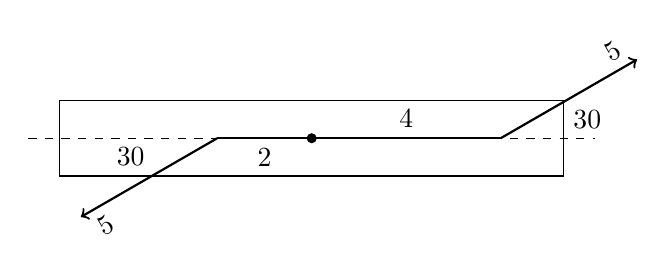
\begin{tikzpicture}[scale=0.8]
        %% Rod
        \draw (-4,-0.6) rectangle (+4,+0.6);
        \draw[dashed] (-4.5,0) -- (4.5,0);
        \draw[fill] (0,0) circle (2pt);
        %% Vectors
        \draw[thick,->] (-1.5,0) -- ++(210:2.5) node[pos=1.0,anchor=north west,rotate=30] {\SI{5}{\newton}};
        \node[anchor=north east] at (-2.5,0) {\ang{30}};
        \draw[thick,->] (3,0) -- ++(30:2.5) node[pos=1.0,anchor=south east,rotate=30] {\SI{5}{\newton}};
        \node[anchor=south west] at (+4,0) {\ang{30}};
        %% Distance
        \draw[thick] (0,0)  -- (+3.0,0) node[anchor=south,pos=0.5] {\SI{4}{\meter}};
        \draw[thick] (0,0)  -- (-1.5,0) node[anchor=north,pos=0.5] {\SI{2}{\meter}};
    \end{tikzpicture}
    \end{center}
    The magnitude of the total torque about the pivot is:
    \begin{multicols}{3}
    \begin{choices}
        \wrongchoice{\SI{0}{\newton\meter}}
        \wrongchoice{\SI{5}{\newton\meter}}
        \wrongchoice{\SI{8.7}{\newton\meter}}
      \correctchoice{\SI{15}{\newton\meter}}
        \wrongchoice{\SI{26}{\newton\meter}}
    \end{choices}
    \end{multicols}
\end{question}
}

\element{halliday-mc}{
\begin{question}{halliday-ch10-q59}
    $\Tau = I\alpha$ for an object rotating about a fixed axis,
        where $\Tau$ is the net torque acting on it,
        $I$ is its rotational inertia, and $\alpha$ is its angular acceleration.
    This expression:
    \begin{choices}
        \wrongchoice{is the definition of torque}
        \wrongchoice{is the definition of rotational inertia}
        \wrongchoice{is the definition of angular acceleration}
      \correctchoice{follows directly from Newton’s second law}
        \wrongchoice{depends on a principle of physics that is unrelated to Newton's second law}
    \end{choices}
\end{question}
}

\element{halliday-mc}{
\begin{question}{halliday-ch10-q60}
    A meter stick on a horizontal frictionless table top is pivoted at the \SI{80}{\centi\meter} mark. 
    It is initially at rest. 
    A horizontal force $\vec{F}_1$ is applied perpendicularly to the end of the stick at \SI{0}{\centi\meter}, as shown. 
    \begin{center}
    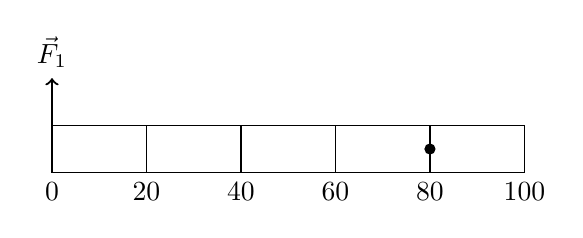
\begin{tikzpicture}[scale=0.6]
        \draw (0,0) rectangle (100mm,10mm);
        \draw[thick,->] (0,0) -- ++(90:2) node[anchor=south] {$\vec{F}_1$};
        \draw[fill] (80mm,5mm) circle (3pt);
        \foreach \i in {0,20,40,60,80,100}{
            \draw (\i mm,10mm) -- (\i mm,0mm) node[anchor=north] {\SI{\i}{\centi\meter}};
        }
    \end{tikzpicture}
    \end{center}
    A second horizontal force $\vec{F}_2$ (not shown) is applied at the \SI{100}{\centi\meter} end of the stick. 
    If the stick does not rotate:
    \begin{choices}
      \correctchoice{$\left| \vec{F}_2 \right| > \left| \vec{F}_1 \right|$ for all orientations of $\vec{F}_2$}
        \wrongchoice{$\left| \vec{F}_2 \right| < \left| \vec{F}_1 \right|$ for all orientations of $\vec{F}_2$}
        \wrongchoice{$\left| \vec{F}_2 \right| = \left| \vec{F}_1 \right|$ for all orientations of $\vec{F}_2$}
        \wrongchoice{$\left| \vec{F}_2 \right| > \left| \vec{F}_1 \right|$ for some orientations of $\vec{F}_2$ and ${\left| \vec{F}_2 \right| < \left| \vec{F}_1 \right|}$ for others}
        \wrongchoice{$\left| \vec{F}_2 \right| > \left| \vec{F}_1 \right|$ for some orientations of $\vec{F}_2$ and ${\left| \vec{F}_2 \right| = \left| \vec{F}_1 \right|}$ for others}
    \end{choices}
\end{question}
}

\element{halliday-mc}{
\begin{question}{halliday-ch10-q61}
    A uniform disk, a thin hoop, and a uniform sphere, all with the same mass and same outer radius,
        are each free to rotate about a fixed axis through its center. 
    Assume the hoop is connected to the rotation axis by light spokes. 
    With the objects starting from rest,
        identical forces are simultaneously applied to the rims, as shown. 
    \begin{center}
    ~\hfill
    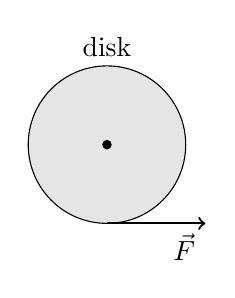
\begin{tikzpicture}
        \draw[fill=white!90!black] (0,0) circle (1);
        \draw[fill] (0,0) circle (1.5pt);
        \node[anchor=south] at (0,1) {disk};
        \draw[thick,->] (0,-1) -- ++(0:1.25) node[anchor=north east] {$\vec{F}$};
    \end{tikzpicture}
    \hfill
    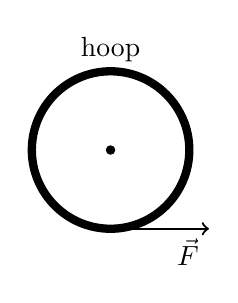
\begin{tikzpicture}
        \draw[line width=3pt] (0,0) circle (1);
        \draw[fill] (0,0) circle (1.5pt);
        \node[anchor=south] at (0,1) {hoop};
        \draw[thick,->] (0,-1) -- ++(0:1.25) node[anchor=north east] {$\vec{F}$};
    \end{tikzpicture}
    \hfill
    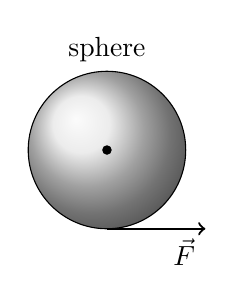
\begin{tikzpicture}
        \draw[shading=ball,ball color=white!90!black] (0,0) circle (1);
        \draw[fill] (0,0) circle (1.5pt);
        \node[anchor=south,] at (0,1) {sphere};
        \draw[thick,->] (0,-1) -- ++(0:1.25) node[anchor=north east] {$\vec{F}$};
    \end{tikzpicture}
    \hfill~
    \end{center}
    Rank the objects according to their angular accelerations,
        least to greatest.
    \begin{choices}
        \wrongchoice{disk, hoop, sphere}
        \wrongchoice{hoop, disk, sphere}
        \wrongchoice{hoop, sphere, disk}
      \correctchoice{hoop, disk, sphere}
        \wrongchoice{sphere, disk, hoop}
    \end{choices}
\end{question}
}

\element{halliday-mc}{
\begin{question}{halliday-ch10-q62}
    A disk is free to rotate on a fixed axis. 
    A force of given magnitude $F$,
        in the plane of the disk, is to be applied. 
    Of the following alternatives the greatest angular acceleration is obtained if the force is:
    \begin{choices}
        \wrongchoice{applied tangentially halfway between the axis and the rim}
      \correctchoice{applied tangentially at the rim}
        \wrongchoice{applied radially halfway between the axis and the rim}
        \wrongchoice{applied radially at the rim}
        \wrongchoice{applied at the rim but neither radially nor tangentially}
    \end{choices}
\end{question}
}

\element{halliday-mc}{
\begin{question}{halliday-ch10-q63}
    A cylinder is \SI{0.10}{\meter} in radius and \SI{0.20}{\meter} in length. 
    Its rotational inertia, about the cylinder axis on which it is mounted,
        is \SI{0.020}{\kilo\gram\meter\squared}.
    A string is wound around the cylinder and pulled with a force of \SI{1.0}{\newton}.
    The angular acceleration of the cylinder is:
    \begin{multicols}{2}
    \begin{choices}
        \wrongchoice{\SI{2.5}{\radian\per\second\squared}}
      \correctchoice{\SI{5.0}{\radian\per\second\squared}}
        \wrongchoice{\SI{10}{\radian\per\second\squared}}
        \wrongchoice{\SI{15}{\radian\per\second\squared}}
        \wrongchoice{\SI{20}{\radian\per\second\squared}}
    \end{choices}
    \end{multicols}
\end{question}
}

\element{halliday-mc}{
\begin{question}{halliday-ch10-q64}
    A disk with a rotational inertia of \SI{2.0}{\kilo\gram\meter\squared}
        and a radius of \SI{0.40}{\meter} rotates on a frictionless
        fixed axis perpendicular to the disk faces and through its center. 
    A force of \SI{5.0}{\newton} is applied tangentially to the rim. 
    The angular acceleration of the disk is:
    \begin{multicols}{2}
    \begin{choices}
        \wrongchoice{\SI{0.40}{\radian\per\second\squared}}
        \wrongchoice{\SI{0.60}{\radian\per\second\squared}}
      \correctchoice{\SI{1.0}{\radian\per\second\squared}}
        \wrongchoice{\SI{2.5}{\radian\per\second\squared}}
        \wrongchoice{\SI{10}{\radian\per\second\squared}}
    \end{choices}
    \end{multicols}
\end{question}
}

\element{halliday-mc}{
\begin{question}{halliday-ch10-q65}
    A disk with a rotational inertia of \SI{5.0}{\kilo\gram\meter\squared}
        and a radius of \SI{0.25}{\meter} rotates on a frictionless
        fixed axis perpendicular to the disk and through its center. 
    A force of \SI{8.0}{\newton} is applied along the rotation axis. 
    The angular acceleration of the disk is:
    \begin{multicols}{2}
    \begin{choices}
      \correctchoice{zero}
        \wrongchoice{\SI{0.40}{\radian\per\second\squared}}
        \wrongchoice{\SI{0.60}{\radian\per\second\squared}}
        \wrongchoice{\SI{1.0}{\radian\per\second\squared}}
        \wrongchoice{\SI{2.5}{\radian\per\second\squared}}
    \end{choices}
    \end{multicols}
\end{question}
}

\element{halliday-mc}{
\begin{question}{halliday-ch10-q66}
    A disk with a rotational inertia of \SI{5.0}{\kilo\gram\meter\squared}
        and a radius of \SI{0.25}{\meter} rotates on a frictionless
        fixed axis perpendicular to the disk and through its center. 
    A force of \SI{8.0}{\newton} is applied tangentially to the rim. 
    If the disk starts at rest,
        then after it has turned through half a revolution its angular velocity is:
    \begin{multicols}{2}
    \begin{choices}
        \wrongchoice{\SI{0.57}{\radian\per\second}}
        \wrongchoice{\SI{0.64}{\radian\per\second}}
        \wrongchoice{\SI{0.80}{\radian\per\second}}
      \correctchoice{\SI{1.6}{\radian\per\second}}
        \wrongchoice{\SI{3.2}{\radian\per\second}}
    \end{choices}
    \end{multicols}
\end{question}
}

\element{halliday-mc}{
\begin{question}{halliday-ch10-q67}
    A thin circular hoop of mass \SI{1.0}{\kilo\gram} and radius \SI{2.0}{\meter}
        is rotating about an axis through its center and perpendicular to its plane. 
    It is slowing down at the rate of \SI{7.0}{\radian\per\second}. 
    The net torque acting on it is:
    \begin{multicols}{2}
    \begin{choices}
        \wrongchoice{\SI{7.0}{\newton\meter}}
        \wrongchoice{\SI{14.0}{\newton\meter}}
      \correctchoice{\SI{28.0}{\newton\meter}}
        \wrongchoice{\SI{44.0}{\newton\meter}}
        \wrongchoice{none of the provided}
    \end{choices}
    \end{multicols}
\end{question}
}

\element{halliday-mc}{
\begin{question}{halliday-ch10-q68}
    A certain wheel has a rotational inertia of \SI{12}{\kilo\gram\meter\squared}.
    As it turns through \SI{5.0}{\revolution} its angular velocity increases from \SI{5.0}{\radian\per\second} to \SI{6.0}{\radian\per\second}.
    If the net torque is constant its value is:
    \begin{multicols}{2}
    \begin{choices}
        \wrongchoice{\SI{0.016}{\newton\meter}}
        \wrongchoice{\SI{0.18}{\newton\meter}}
        \wrongchoice{\SI{0.57}{\newton\meter}}
      \correctchoice{\SI{2.1}{\newton\meter}}
        \wrongchoice{\SI{3.6}{\newton\meter}}
    \end{choices}
    \end{multicols}
\end{question}
}

\element{halliday-mc}{
\begin{question}{halliday-ch10-q69}
    A \SI{16}{\kilo\gram} block is attached to a cord that is wrapped around the rim of a flywheel of diameter \SI{0.40}{\meter} and hangs vertically, as shown.
    \begin{center}
    \begin{tikzpicture}
        %% Ceiling
        \node[anchor=south,fill,pattern=north east lines,minimum width=4cm, minimum height=0.05cm] at (0,0) {};
        \draw (-2,0) -- (2,0);
        %% Pulley
        \draw[thick] (0,-1.5) circle (1);
        \draw[fill=white!80!black] (-0.5,0) -- (-0.25,-1.6) arc(190:350:0.25) -- (0.5,0) -- cycle;
        \draw[fill] (0,-1.5) circle (1.5pt);
        \draw[thick,<->] (-1.75,-0.5) -- (-1.75,-2.5) node[pos=0.5,anchor=center,fill=white] {\SI{0.4}{\meter}};
        %% Mass
        \node[draw,fill=white!90!black,minimum size=1.0cm,anchor=south] (M) at (1,-4) {\SI{16}{\kilo\gram}};
        %% Rope
        \draw[thick] (M.north) -- (1,-1.5);
    \end{tikzpicture}
    \end{center}
    The rotational inertia of the flywheel is \SI{0.50}{\kilo\gram\meter\squared}.
    When the block is released and the cord unwinds,
        the acceleration of the block is:
    \begin{multicols}{3}
    \begin{choices}
        \wrongchoice{$0.15 g$}
      \correctchoice{$0.56 g$}
        \wrongchoice{$0.84 g$}
        \wrongchoice{$g$}
        \wrongchoice{$1.3 g$}
    \end{choices}
    \end{multicols}
\end{question}
}

\element{halliday-mc}{
\begin{question}{halliday-ch10-q70}
    A \SI{8.0}{\centi\meter} radius disk with a rotational inertia of \SI{0.12}{\kilo\gram\meter\squared} is free to rotate on a horizontal axis.
    A string is fastened to the surface of the disk and a \SI{10}{\kilo\gram} mass hangs from the other end.
    The mass is raised by using a crank to apply a \SI{9.0}{\newton\meter} torque to the disk.
    The acceleration of the mass is:
    \begin{multicols}{3}
    \begin{choices}
        \wrongchoice{\SI{0.50}{\meter\per\second\squared}}
        \wrongchoice{\SI{1.7}{\meter\per\second\squared}}
        \wrongchoice{\SI{6.2}{\meter\per\second\squared}}
        \wrongchoice{\SI{12}{\meter\per\second\squared}}
        \wrongchoice{\SI{20}{\meter\per\second\squared}}
    \end{choices}
    \end{multicols}
\end{question}
}

\element{halliday-mc}{
\begin{question}{halliday-ch10-q71}
    A \SI{0.70}{\kilo\gram} disk with a rotational inertia given by $M R^2/2$ is free to rotate on a fixed horizontal axis suspended from the ceiling. 
    A string is wrapped around the disk and a \SI{2.0}{\kilo\gram} mass hangs from the free end. 
    If the string does not slip,
        then as the mass falls and the cylinder rotates,
        the suspension holding the cylinder pulls up on the cylinder with a force of:
    \begin{multicols}{3}
    \begin{choices}
        \wrongchoice{\SI{6.9}{\newton}}
      \correctchoice{\SI{9.8}{\newton}}
        \wrongchoice{\SI{16}{\newton}}
        \wrongchoice{\SI{26}{\newton}}
        \wrongchoice{\SI{29}{\newton}}
    \end{choices}
    \end{multicols}
\end{question}
}

\newcommand{\hallidayChTenQSeventyTwo}{
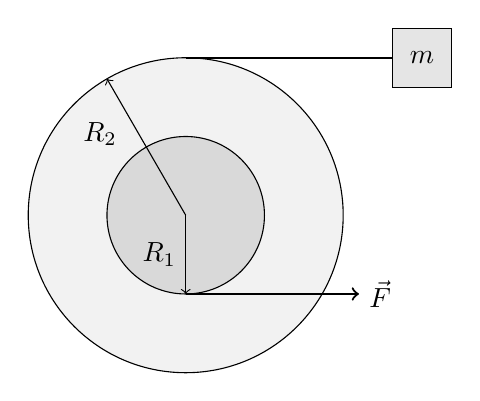
\begin{tikzpicture}
    %% Circles
    \draw[fill=white!95!black] (0,0) circle (2cm);
    \draw[fill=white!85!black] (0,0) circle (1cm);
    %% Radii
    \draw[->] (0,0) -- (270:1cm) node[pos=0.5,anchor=east] {$R_1$};
    \draw[->] (0,0) -- (120:2cm) node[pos=0.75,anchor=north east] {$R_2$};
    %% Force
    \draw[thick,->] (0,-1) -- ++(0:2.2cm) node[anchor=west] {$\vec{F}$};
    %% mass
    \node[draw,minimum size=0.75cm,fill=white!90!black,anchor=center] (M) at (3,2) {$m$};
    \draw[thick] (0,2) -- (M.west);
\end{tikzpicture}
}

\element{halliday-mc}{
\begin{question}{halliday-ch10-q72}
    A small disk of radius $R_1$ is mounted coaxially with a larger disk of radius $R_2$. 
    The disks are securely fastened to each other and the combination is free to rotate on a fixed axle that is perpendicular to a horizontal frictionless table top, as shown in the overhead view below.
    The rotational inertia of the combination is $I$. 
    A string is wrapped around the larger disk and attached to a block of mass $m$, on the table. 
    Another string is wrapped around the smaller disk and is pulled with a force $F$ as shown. 
    \begin{center}
        \hallidayChTenQSeventyTwo
    \end{center}
    The acceleration of the block is:
    \begin{multicols}{2}
    \begin{choices}
        \wrongchoice{$\dfrac{R_1 F}{mR_2}$}
        \wrongchoice{$\dfrac{R_1 R_2 F}{I - mR_2^2}$}
      \correctchoice{$\dfrac{R_1 R_2 F}{I + mR_2^2}$}
        \wrongchoice{$\dfrac{R_1 R_2 F}{I - mR_1 R_2}$}
        \wrongchoice{$\dfrac{R_1 R_2 F}{I + mR_1 R_2}$}
    \end{choices}
    \end{multicols}
\end{question}
}

\element{halliday-mc}{
\begin{question}{halliday-ch10-q73}
    A small disk of radius $R_1$ is mounted coaxially with a larger disk of radius $R_2$. 
    The disks are securely fastened to each other and the combination is free to rotate on a fixed axle that is perpendicular to a horizontal frictionless table top, as shown in the overhead view below.
    The rotational inertia of the combination is $I$. 
    A string is wrapped around the larger disk and attached to a block of mass $m$, on the table. 
    Another string is wrapped around the smaller disk and is pulled with a force $F$ as shown. 
    \begin{center}
        \hallidayChTenQSeventyTwo
    \end{center}
    The tension in the string pulling the block is:
    \begin{multicols}{2}
    \begin{choices}
        \wrongchoice{$\dfrac{R_1 F}{R_2}$}
        \wrongchoice{$\dfrac{m R_1 R_2 F}{I - mR_2^2}$}
      \correctchoice{$\dfrac{m R_1 R_2 F}{I + mR_2^2}$}
        \wrongchoice{$\dfrac{m R_1 R_2 F}{I - mR_1 R_2}$}
        \wrongchoice{$\dfrac{m R_1 R_2 F}{I + mR_1 R_2}$}
    \end{choices}
    \end{multicols}
\end{question}
}

\element{halliday-mc}{
\begin{question}{halliday-ch10-q74}
    A block is attached to each end of a rope that passes over a pulley suspended from the ceiling.
    The blocks do not have the same mass. 
    If the rope does not slip on the pulley,
        then at any instant after the blocks start moving, the rope:
    \begin{choices}
      \correctchoice{pulls on both blocks, but exerts a greater force on the heavier block}
        \wrongchoice{pulls on both blocks, but exerts a greater force on the lighter block}
        \wrongchoice{pulls on both blocks and exerts the same magnitude force on both}
        \wrongchoice{does not pull on either block}
        \wrongchoice{pulls only on the lighter block}
    \end{choices}
\end{question}
}

\element{halliday-mc}{
\begin{question}{halliday-ch10-q75}
    A pulley with a radius of \SI{3.0}{\centi\meter} and a rotational inertia of \SI{4.5e-3}{\kilo\gram\meter\squared} is suspended from the ceiling. 
    A rope passes over it with a \SI{2.0}{\kilo\gram} block attached to one end and a \SI{4.0}{\kilo\gram} block attached to the other. 
    The rope does not slip on the pulley. 
    When the speed of the heavier block is \SI{2.0}{\meter\per\second} the kinetic energy of the pulley is:
    \begin{multicols}{3}
    \begin{choices}
        \wrongchoice{\SI{0.15}{\joule}}
        \wrongchoice{\SI{0.30}{\joule}}
        \wrongchoice{\SI{1.0}{\joule}}
        \wrongchoice{\SI{10}{\joule}}
        \wrongchoice{\SI{20}{\joule}}
    \end{choices}
    \end{multicols}
\end{question}
}

\element{halliday-mc}{
\begin{question}{halliday-ch10-q76}
    A pulley with a radius of \SI{3.0}{\centi\meter} and a rotational inertia of \SI{4.5e-3}{\kilo\gram\meter\squared} is suspended from the ceiling. 
    A rope passes over it with a \SI{2.0}{\kilo\gram} block attached to one end and a \SI{4.0}{\kilo\gram} block attached to the other. 
    The rope does not slip on the pulley. 
    At any instant after the blocks start moving,
        the object with the greatest kinetic energy is:
    \begin{choices}
        \wrongchoice{the heavier block}
        \wrongchoice{the lighter block}
      \correctchoice{the pulley}
        \wrongchoice{either block (the two blocks have the same kinetic energy)}
        \wrongchoice{none (all three objects have the same kinetic energy)}
    \end{choices}
\end{question}
}

\element{halliday-mc}{
\begin{question}{halliday-ch10-q77}
    A disk with a rotational inertia of \SI{5.0}{\kilo\gram\meter\squared} and a radius of \SI{0.25}{\meter} rotates on a fixed axis perpendicular to the disk and through its center.
    A force of \SI{2.0}{\newton} is applied tangentially to the rim. 
    As the disk turns through half a revolution the work done by the force is:
    \begin{multicols}{3}
    \begin{choices}
      \correctchoice{\SI{1.6}{\joule}}
        \wrongchoice{\SI{2.5}{\joule}}
        \wrongchoice{\SI{6.3}{\joule}}
        \wrongchoice{\SI{10}{\joule}}
        \wrongchoice{\SI{40}{\joule}}
    \end{choices}
    \end{multicols}
\end{question}
}

\element{halliday-mc}{
\begin{question}{halliday-ch10-q78}
    A circular saw is powered by a motor. 
    When the saw is used to cut wood, the wood exerts a torque of \SI{0.80}{\newton\meter} on the saw blade. 
    If the blade rotates with a constant angular velocity of \SI{20}{\radian\per\second} the work done on the blade by the motor in \SI{1.0}{\minute} is:
    \begin{multicols}{3}
    \begin{choices}
        \wrongchoice{zero}
        \wrongchoice{\SI{480}{\joule}}
      \correctchoice{\SI{960}{\joule}}
        \wrongchoice{\SI{1400}{\joule}}
        \wrongchoice{\SI{1800}{\joule}}
    \end{choices}
    \end{multicols}
\end{question}
}

\element{halliday-mc}{
\begin{question}{halliday-ch10-q79}
    A disk has a rotational inertia of \SI{6.0}{\kilo\gram\meter\squared} and a constant angular acceleration of \SI{2.0}{\radian\per\second\squared}.
    If it starts from rest the work done during the first \SI{5.0}{\second} by the net torque acting on it is:
    \begin{multicols}{3}
    \begin{choices}
        \wrongchoice{zero}
        \wrongchoice{\SI{30}{\joule}}
        \wrongchoice{\SI{60}{\joule}}
      \correctchoice{\SI{300}{\joule}}
        \wrongchoice{\SI{600}{\joule}}
    \end{choices}
    \end{multicols}
\end{question}
}

\element{halliday-mc}{
\begin{question}{halliday-ch10-q80}
    A disk starts from rest and rotates around a fixed axis,
        subject to a constant net torque. 
    %% change wording to include ``interval''
    The work done by the torque during the second \SI{5}{\second} interval is
        \rule[-0.1pt]{4em}{0.1pt} as the work done during the first \SI{5}{\second} interval.
    \begin{choices}
        \wrongchoice{the same}
        \wrongchoice{twice as much}
        \wrongchoice{half as much}
      \correctchoice{four times as much}
        \wrongchoice{one-fourth as much}
    \end{choices}
\end{question}
}

\element{halliday-mc}{
\begin{question}{halliday-ch10-q81}
    A disk starts from rest and rotates about a fixed axis,
        subject to a constant net torque. 
    The work done by the torque during the second revolution is
        \rule[-0.1pt]{4em}{0.1pt} as the work done during the first revolution.
    \begin{choices}
      \correctchoice{the same}
        \wrongchoice{twice as much}
        \wrongchoice{half as much}
        \wrongchoice{four times as much}
        \wrongchoice{one-fourth as much}
    \end{choices}
\end{question}
}


\endinput


